\documentclass{article}
\usepackage{graphicx}
\usepackage[margin=1in]{geometry}
\usepackage{subcaption}
\usepackage{csvsimple}
\usepackage{booktabs}
\usepackage{pgfplotstable} %for making tables from csv files
\usepackage{longtable} %to fix my long table
\usepackage{tabu} % if you want - to fix a wide table

\begin{document}

\title{Simulation Write Up{}}
\author{Amy Solman}

\maketitle

\section{Aims}
To test the hypothesis that the predictions made by Chisholm’s model are significantly statistically similar to the results of the island simulation. \bigskip

\noindent To test the hypothesis that, as island area increases, it transitions from a niche-structured regime, to a colonisation-extinction balance regime. 

\section{Methods}

\subsection{Simulation Design}

\subsubsection{Overview}
This simulation is designed to mimic the process of island colonisation from a metacommunity (size = 10 000). The colonisation process is constrained by a fixed speciation rate (0.001) within the local community, as the metacommunity is considered to be static throughout the simulation. The colonisation process is also constrained by migration rate . Each island is characterised by number of niches and the size of each niche. The output of the simulation is the final community of each island as well as a timeseries of species richness recorded every 10 000 timesteps. 

\subsubsection{Metacommunity}
A metacommunity is generated at the beginning of the simulation using \textit{coalescence\_test} function, provided by Dr James Rosindell. The function takes the input parameters: metacommunity size(\textit{J\_meta}) and speciation rate (\textit{nu}). It initialises a vector (\textit{lineages}) of length(\textit{J\_meta}) with 1 as every value. An empty vector (\textit{abundances}) is initialised. The value of \textit{J\_meta} is given to \textit{N}. \textit{Theta} is calculated as \textit{nu*(J\_meta-1)/(1-nu)}. Then, while \textit{N $>$ 1}, a vector \textit{linvect} is created with values 1:length\textit{J\_meta}. A random sample of \textit{linvect} is made (\textit{j}). A random decimal number is selected between 0 and 1 (\textit{randnum}. If \textit{rannum} is less than \textit{theta/(theta+N-1)}, then the value at \textit{lineages[j]} is appended to \textit{abundances}. Else, another random number (\textit{i}) is sampled from \textit{linvect}, excluding the last number selected. The values at \textit{lineages[i]} and \textit{lineages[j]} are summed and take the position of \textit{lineages[i]}. \textit{lineages[j]} is then removed from \textit{lineages}, so the vector is one value shorter. The value of \textit{N} is also decreased by 1. This repeats until \textit{N} !$>$ 1. The remaining value in the \textit{lineages} vector is added to \textit{abundances} and the function outputs a vector of simulated species abundances.\bigskip

\noindent The \textit{coalescence\_test} function is incorporated into a second function (\textit{metacommunity}), that generates a vector of individuals from the abundance vector. For example, \textit{abundances}(5, 4, 2, 2, 1, 1) would generate a community \textit{meta}(1,1,1,1,1,2,2,2,2,3,3,4,4,5,6) where each unique number value represents a unique species.\bigskip     

\subsubsection{Parameters}
The variables parameters of the simulation are: migration rate (range: 0.003-0.06), number of niches (range: 1-20), size of niches (range:1-20). Each unit of space was assumed to host one individual, therefore, number of niches x size of niches = area = size of island population. There were a total of 400 difference condition combinations applied during the simulation (see Appendix). 


\subsubsection{Simulation Logic}
I developed a simulation which took the inputs of meta community size (J\_meta), speciation rate (nu), the number of different migration rates to be simulated (num\_m\_rates), the maximum niche size (max\_k\_size), the maximum number of niches to be simulated (max\_k\_num), the amount of time the simulation is to be run for (wall\_time) and the name of the files in which to store the simulation data (output\_file\_name).\bigskip

For each simulation I began by generating a metacommunity, using the function coalescence\_test written by James Rosindell. The function took the inputs of J\_meta and nu, and output a vector of simulated species abundances. I passed the abundance vector to a second function (metacommunity), that repeated a unique species number by each number of the abundance vector (for example abundance vector (5,4,1,1) gives community (1,1,1,1,1,2,2,2,2,3,4)). \bigskip

The size of each simulation island was determined by the number of niches multiplied by the size of each niche. Each niche on each island was generated through the niche\_info function. The function took the inputs of migration rate (m), speciation rate (nu) and niche size (k\_size). Each niche started off with a completely homogenous community of species 1 by k\_size (for example k\_size = 5, niche community = 1,1,1,1,1). The starting community of each niche, as well as speciation and migration rate were stored in an output list. The niche\_info function run through the niches function, and repeated from 1 to maximum niche size (max\_k\_num), outputting island communities that grew in size from one niche to max\_k\_num (for example, max\_k\_num = 3 would produce 3 islands consisting of 1 niche, 2 niches and 3 niches, each of k\_size). \bigskip

The niches function was repeated through the multi\_islands function, from 1 to the number of different migration rates (num\_m\_rates). Migration rates started at 0.002 and increased by 0.002 each time. The multi\_islands function also generated a unique species list (unique\_sp) that calculated the number of unique species across all niches of each islands and stored this data, along with each island community, speciation and migration rate. The output of multi\_islands was a list of islands, along with the communities of each of their niches, the speciation and migration rates of each niche, and the total number of unique species on that island. \bigskip
 
 \begin{figure}[h!]
\centering
  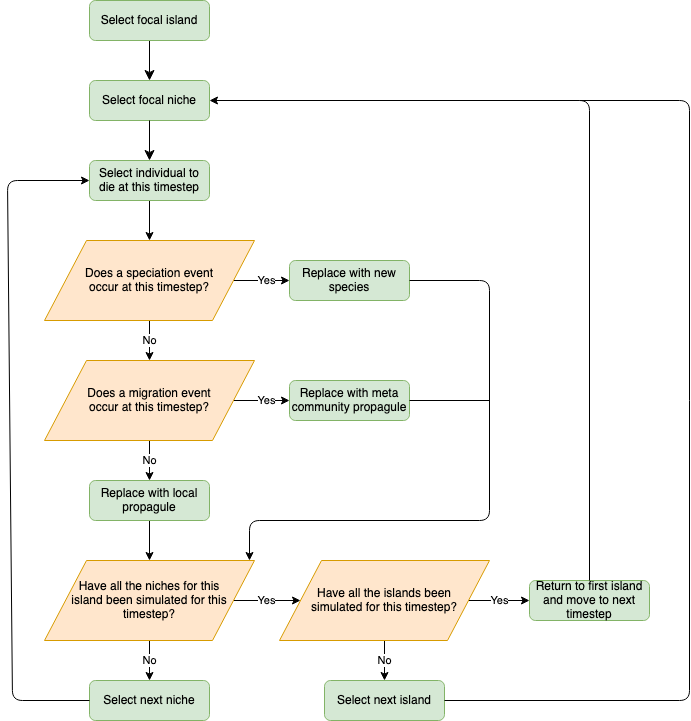
\includegraphics[scale=0.4]{../../Other/neutral_flowchart.png}
  \caption{Flowchart of simulation design}
  \label{fig:Flowchart}
\end{figure}
 
I then started a timer. While the timer was less than the wall\_time the cluster\_run\_function would continue to loop through the communities. At each time step, each island is chosen and each niche is passed through the simulation\_one\_timestep function.  An individual within that niche chosen to die and with probability speciation (0.001) a new species is generated to take its place. With probability migration rate, an individual chosen from the metacommunity replaces the dead individual. With probability 1 – speciation rate + migration rate, an individual is chosen from within the niche to replace the dead individual. Once all niches for one island have had simulation\_one\_timestep act upon it, the simulation moves to the next island. Once all niches on all islands have passed through simulation\_one\_timestep, the simulation moves to the next timestep. Every 10000 timesteps the species richness of each island is recorded and stored. The simulation continues until wall\_time is reached. Each run of the cluster\_run\_function output the final communities of each island and a timeseries of species richness, along with the number of timesteps the simulation had progressed through, the total time spent on the simulation, the size of the metacommunity, the speciation rate and the output file name). \bigskip

\subsubsection{High Performance Computing}
A second R script (ClusterCode.R) was written to source the ClusterSim.R functions. The cluster job index number was applied to the value iter. The value iter was given to i and i was used to set a seed for the simulation. Output\_file\_name was given the value of simulation\_timeseries\_i, to give a different output filename for each iteration of the simulation. The cluster\_run\_function was then called (see Table 1 for input parameters). \bigskip

Finally, a bash script (ClusterRun.sh) was used to set the wall\_time for the simulation in the cluster (24:00:00). This script called the ClusterCode.R script to run on the cluster, and output the 100 simulation output files to \$HOME directory. \bigskip

I ran my simulation on the Imperial College London high-performance computing cluster for 23 hours. The simulation was repeated 100 times. Each simulation generated 3375 islands (num\_m\_rates x max\_k\_size x max\_k\_num). 

\subsection{Data Preparation and Timeseries Plots}
After downloading my simulation results from the cluster, I imported each file into DataPrep.R script. I isolated the data from each island and create a data frame with simulation number, migration rate, area, number of niches and number of species. I created a second data frame with simulation number, island number, migration rate, timestep and species richness timeseries for each island. I then saved the final island data and timeseries data to separate csv files. \bigskip

To ensure the simulation had run long enough for each island to reach dynamic equilibrium I wrote a timeseries plotting script (TimeseriesPlot.R). I loaded the R packages GGPlot2 and gridExtra to create my timeseries plots and put save multiple plots to one pdf file respectively. I imported the timeseries data from my simulations (SimTimeseriesPlotData.csv). I then isolated the data from simulations 25, 50 and 75. I plotted the timeseries data of each island for each simulation, on a three-panel plot.  

\section{Analysis}
For my analysis script (Analysis.R), I loaded the R package broom, to use the tidy() function for accessing the summary statistics of linear models. I imported my final island data (SimModelFitData.csv) and for each island across all my simulations (337,500) I generated an estimated species richness by giving the island area, number of niches, m0 and an estimated theta to the chisholm\_function. The results of my simulation and those estimated by the chisholm\_function was then bound together in a data frame. I also found the mean species richness results for each combination of island area, migration rate and number of niches across all 100 simulations.
  
\subsection{Within Simulation Analysis}

\subsubsection{Repeatability}
I checked the repeatability of my simulation by running a linear model of species richness, with simulation number as independent variable. I then run an ANOVA (analysis of variance) on the linear model of species richness with simulation as the explanatory variance. From this I was able to calculate the repeatability statistic. This is calculated by dividing the among-group variance by the within-group variance, minus the among-group variance. We are calculating the percentage of the total variance that is explained by among-simulation differences. Essentially, we want to make sure there is more within simulation variance than among simulation variance. We want to make sure our simulations are relatively consistent. As the same statistical parameters are being applied to each (speciation rate = 0.001, migration rates 0.003 - 0.045, niche numbers 1-15, niche sizes 1-15) we would expect variation among simulations to be less than variation within simulations. We would expect our simulations to give us consistent results. This allowed me to ascertain to what extent the variability in species richness is explained by differences in the simulations.

\subsubsection{Normaility}
I checked the normality of my simulation data by creating histograms of species richness results. It was necessary to check the normality of my data as I use linear regression in my analysis and it assumes the data are normally distributed. 

\subsubsection{Collinearity}
I assessed the collinearity of my simulation dataset by using the R base function pairs() to produce a scatterplot of matrices. This allowed for visual inspection of the relationships between number of species, migration rate, island area and number of niches. It is important to assess the collinearity of covariates because it can inflate variation. Large amounts of collinearity cause covariates to have larger standard errors and it becomes less likely to detect a significant result. The Variance Inflation Factor (VIF) was calculated to assess if the collinearity between number of niches and island area was within acceptable limits for this analysis. 

\subsubsection{Linear Regression}
Next, I began to assess whether there was a statistically significant relationship between my dependent variable (species richness) and independent variables (area and niches). Firstly, I calculated the mean species richness for each unique set of parameters across all 100 simulations. Then, I z-transformed my area and niche variables so that they could better meet the assumptions of a linear model. Moreover, the intercept statistic for z-standardized data gives us the mean of the dependent sample. I ran a linear model on the mean species data and z-transformed area and niche variables separately, to assess to what extent each explained variation in the dependent variable. I also generated histograms of the residuals of each linear model to check for homogeneity of the variances to validate the assumptions of the regression analyses. I then validated the models by checking the distribution of the residuals. 

\subsubsection{Multivariate Analysis}
I performed a multivariate analysis of the mean simulation data, including number of niches, island area and migration rate. This allowed me to assess to what extent the three independent variables were important for predicting species richness. I performed a second multivariate analysis, including niche number and island area only. I plotted the results of both of these models to check the distribution of the residuals.

\subsection{Simulation/Model Analysis}

\subsubsection{Outliers}
For my analysis, I began by checking the data for outliers. I did this by creating boxplots of species richness’s generated by my simulation and those generated by the chisholm\_function. By ensuring the number of possible outliers is low in comparison to sample size, I ensured the data would not be skewed by anomalous results.

\subsubsection{Range, variance, standard deviation and standard error}
I found the range, variance, standard deviation and standard error of both my simulation and the chisholm\_function. Homogeneity of variances is an important assumption for certain statistical tests such as ANOVA and regression analysis. In my analysis I will be working mostly with regression analysis, wherein it is more important to look at the variances of the residuals. 

\subsubsection{Paired-sample t-Test}
A paired-sample t-test was used to assess whether the mean difference between the simulation results and chisholm\_function estimates was zero. I used a paired-sample t-test because both sets of species richness data were calculated from the same set of parameters (migration rate, number of niches, island area) and were, therefore, directly comparable across pairs. 

\subsubsection{Non-Linear Least Squares Fitting}
As well as calculating estimated species richness of each island by calling the chisholm\_function and feeding it the know independent parameters, I also fit the model to the data using Non-linear least squares (NLLS) fitting. I found the mean number species for each area value and fit the model with starting estimations for theta, migration rate and number of niches. 

\subsection{Repeat Analysis with Reducing Data Set}

\begin{table}[ht]
\caption{Reducing dataset to smaller islands}
\centering
    \begin{tabular}{l|l}%
    \bfseries Max Island Size & \bfseries Num. Islands% specify table head
    \csvreader[head to column names]{../../Results/Simulation/DividedDF.csv}{}% use head of csv as column names
    {\\\hline\csvcoli&\csvcolii}% specify your coloumns here
    \end{tabular}
    \end{table}

All analysis was repeated 10 times whilst reducing maximum island area (Table 1). This allowed for comparison of multivariate analysis, to ascertain if the relative significance of the independent parameters changed as island area decreased. I was also able to assess whether the model was better at predicting species richness on smaller verses larger islands.

All analysis and plotting were carried out using R 3.6.0.


\section{Results}

\begin{figure}[!h]
\centering
  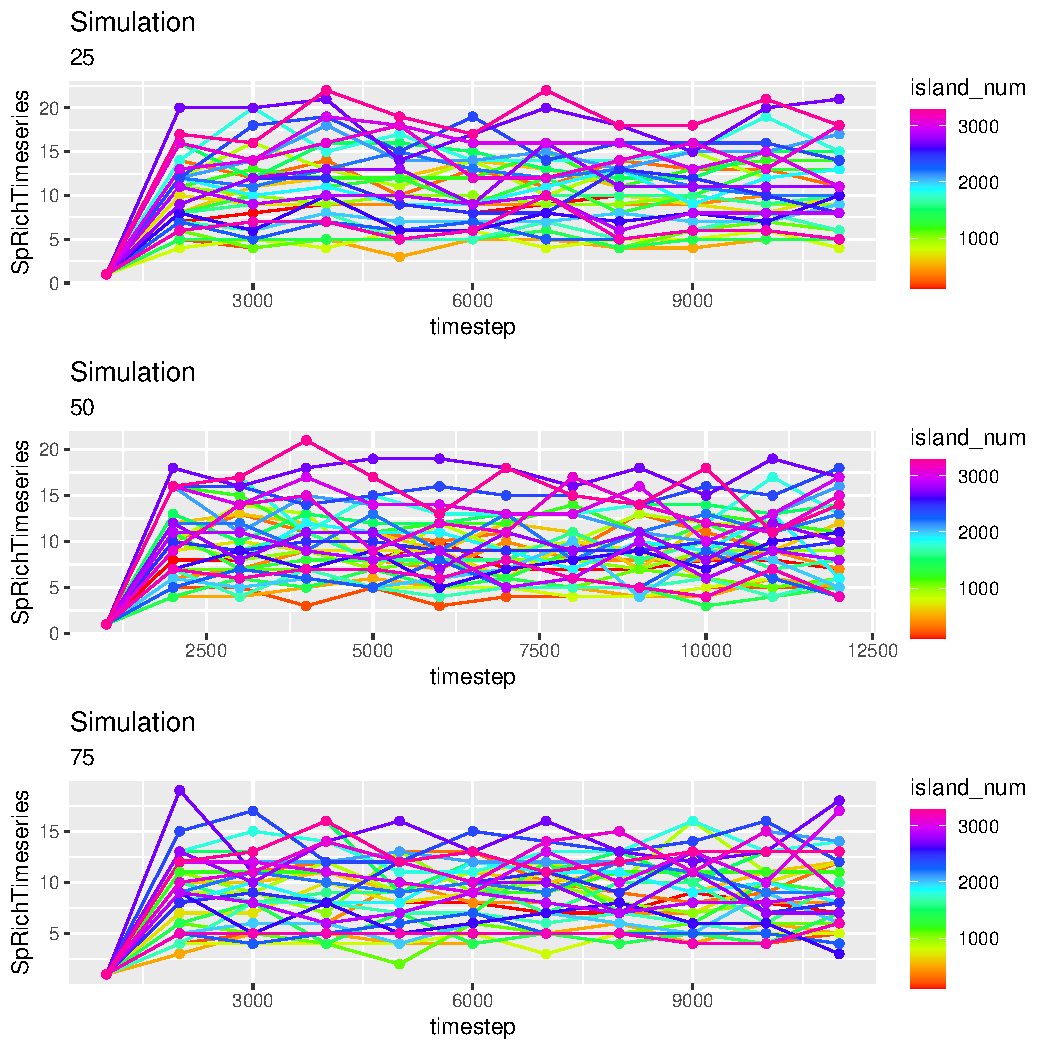
\includegraphics[scale=0.5]{../../Results/Simulation/TimeseriesPlot.pdf}
  \caption{Timeseries plot of three simulations}
  \label{fig:Timeseries plot}
\end{figure}

I used data from 3375 different combinations of parameters (15 migration rates, 15 number of niches, 15 size niches), repeated for 100 simulations, with a total of 337 500 simulated islands. 

\subsection{Within Simulation Results}

\subsection{Timeseries}
3 of 100 simulation were selected and plotted as a timeseries (Figure 2). From this plot it was determined that the islands reached dynamic equilibrium at approximately 25 000 timesteps. 

\subsubsection{Repeatability} %Not entirely sure on repeatability, is this right?
The mean sum of squared variance among simulations was 1059 (Vg). The mean sum of squared variance within simulations was 15.2 (Vr). The repeatability of the simulations was calculated as Vg / (Vg + Vr)  = 0.986. 99\% of the variation in species richness is determined by between-simulation differences. The simulations are giving consistent values of species richness. 

\subsubsection{Collinearity}

\begin{figure}[!h]
  \centering
  \begin{subfigure}[b]{0.4\linewidth}
    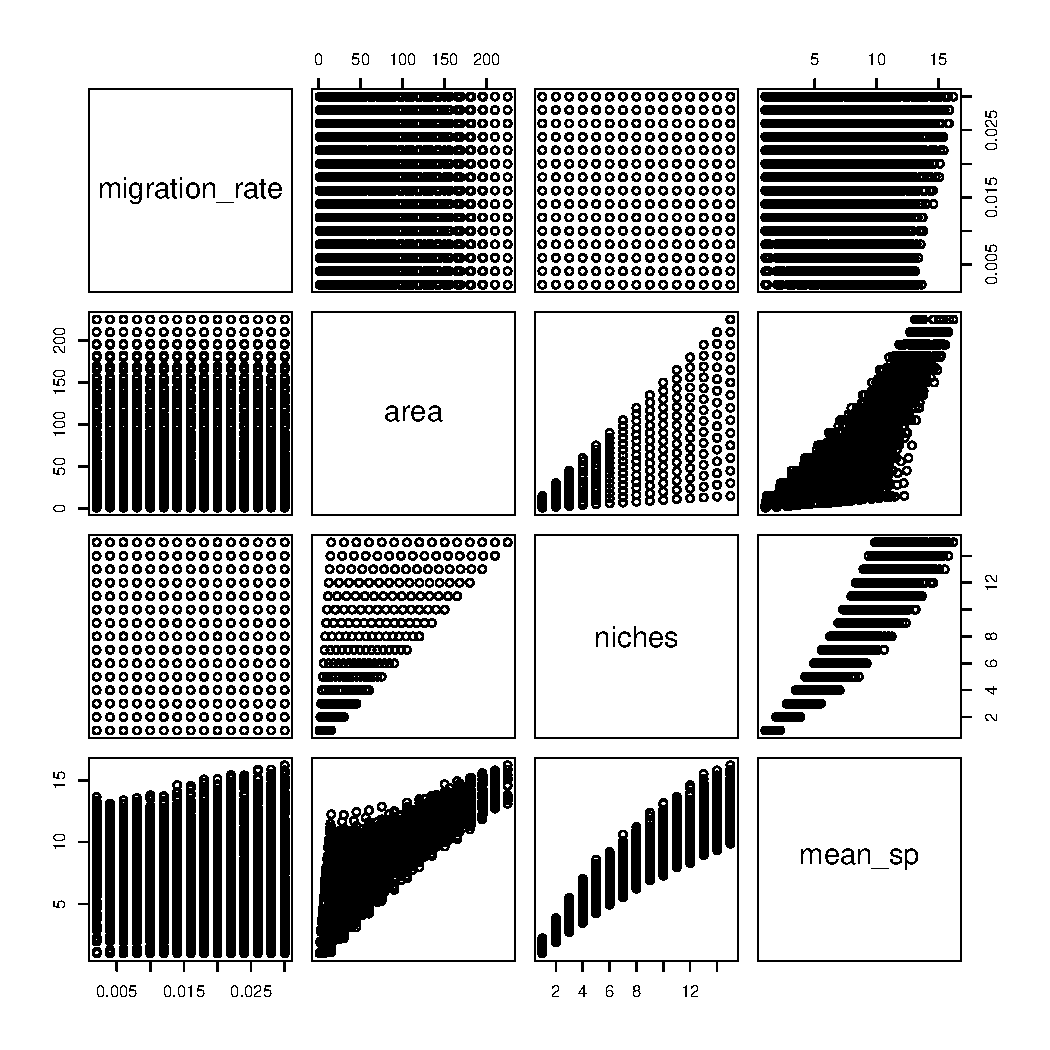
\includegraphics[width=\linewidth]{../../Results/Simulation/CollinearityPlot_1.pdf}
    \caption{maxArea = 225 units}
  \end{subfigure}
  \begin{subfigure}[b]{0.4\linewidth}
    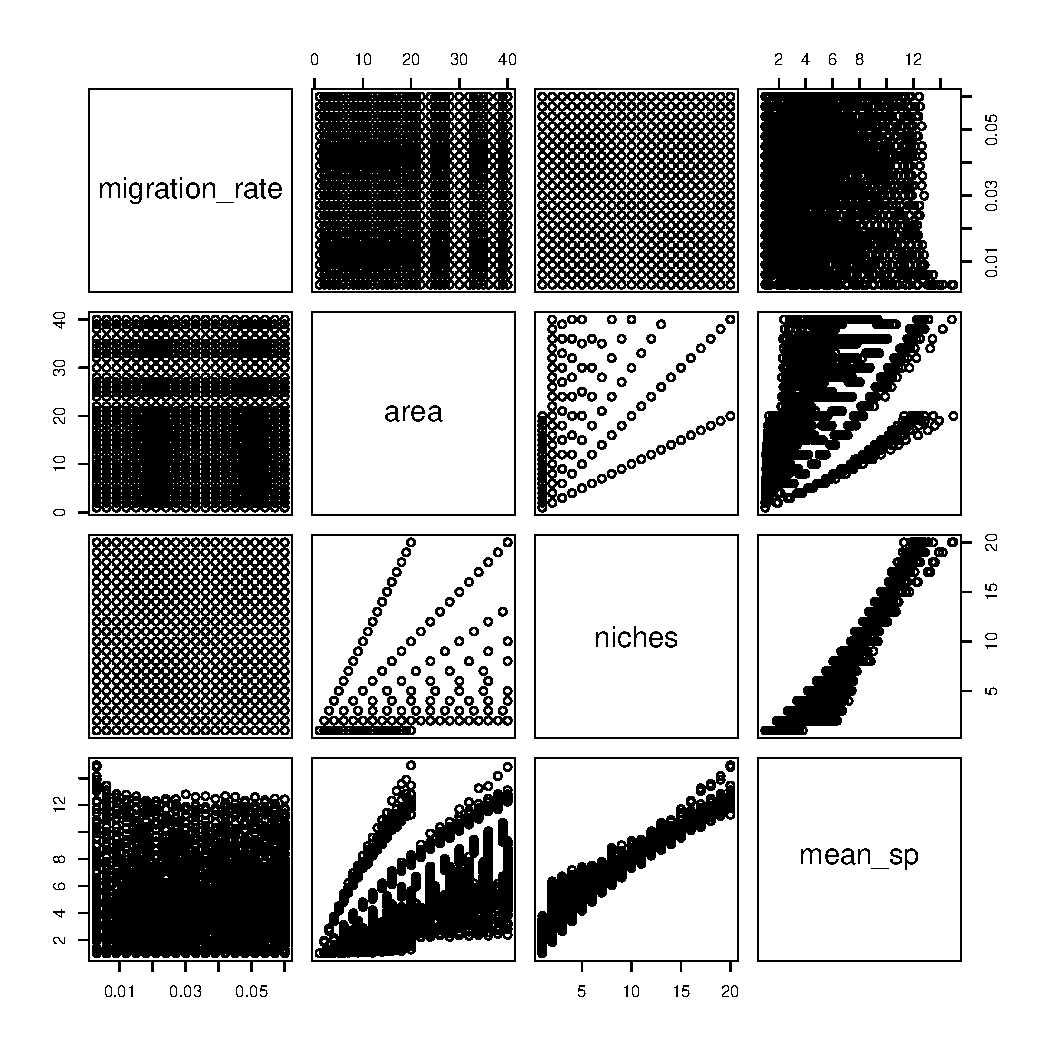
\includegraphics[width=\linewidth]{../../Results/Simulation/CollinearityPlot_10.pdf}
    \caption{maxArea = 22 units}
  \end{subfigure}
  \caption{Collinearity plots for full data set (a) and reduced data set (b)}
  \label{fig:Collinearity}
\end{figure}

The collinearity statistic for migration rate and area, as well as migration rate and niches was 0. A lack of collinearity between migration rate and the other covariates is to be expected as they are not logically linked in the simulation, nor would they be in a real-world scenario. Area and niches had a collinearity score of 0.661. The VIF score for collinearity between niches and area was 1.77. The standard errors of number of niches are therefore inflated by $\sqrt{1.77}$ = 1.33, which is within an acceptable range. 
The collinearity statistic for migration rate and area, as well as migration rate and niches in the most reduced dataset was 0. Area and niches had a collinearity score of 0.306. This is less than that of the whole dataset and therefore in an acceptable range. Visual inspection of pairs plots (Figure 3) supported the collinearity statistics. 

\subsubsection{Linear Regression Analysis}

\begin{table}[h!]
\centering
\caption{Linear regression results for z-transformed area and niches}
\pgfplotstabletypeset[
    col sep=comma,
    ignore chars={",_}, %get rid of quote marks around my text and ignore underscores
    string type,
    every head row/.style={%
        before row={\hline
           % \multicolumn{2}{c}{incase you wanted a title above the column headers} & \\
        },
        after row=\hline
    },
    every last row/.style={after row=\hline},
    columns/maxArea/.style={column name=maxArea, column type=c},
    columns/Coefficients/.style={column name=Coefficients, column type=c},
    columns/Estimate/.style={column name=Estimate, column type=c},
    columns/standarderror/.style={column name=StandardError, column type=c},
    columns/tvalue/.style={column name=tValue, column type=c},
    columns/pvalue/.style={column name=pValue, column type=l}, %problem with less than sign
    columns/rsquared/.style={column name=rSquared, column type=c},
    columns/variate/.style={column name=Variate, column type=l},
    ]{../../Results/Simulation/LMMaxMin.csv}
   \end{table}\bigskip

\begin{figure}[h!]
\centering
  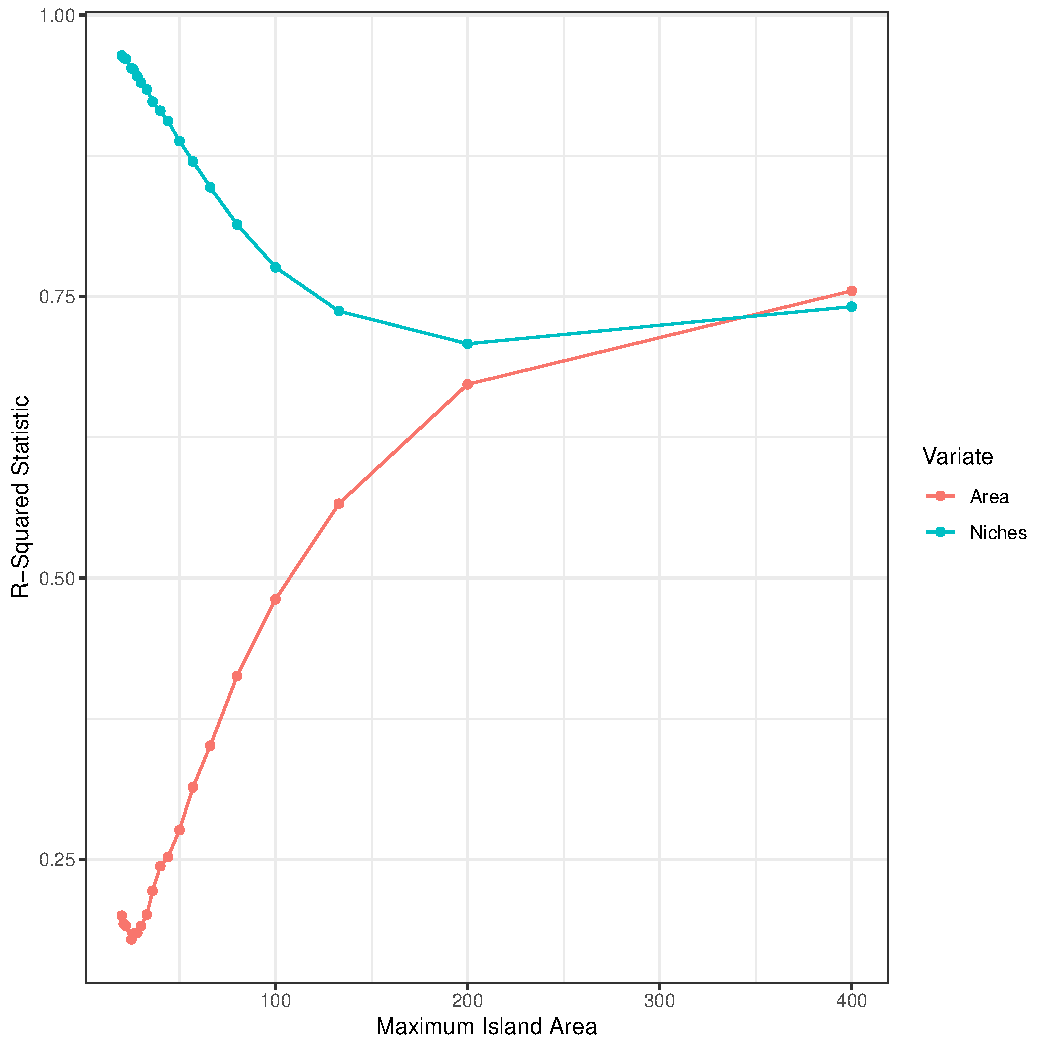
\includegraphics[scale=0.5]{../../Results/Simulation/LMRSquared.pdf}
  \caption{Change of R-squared statistic for number of niches and island area, with changing island size}
  \label{fig:R-Squared statistic}
\end{figure}

The linear model results of species richness and z-transformed area gave an r-squared value of 0.679 with a p-value $<$ 0.001 (Table 2). This indicated that area was a positive, statistically significant relationship between area and species richness for the entire dataset. \bigskip

Visual inspection of residual vs fitted results for the entire dataset shows fairly linear but non-constant variance (Figure 5 (a)). Lower fitted values had a greater residual range than higher fitted values. The normal Q-Q plot showing standardised residuals plotted against the quantiles they are supposed to lie in fall along a relatively straight line. Diagnostics indicate the model works fairly well for the data.  \bigskip

The r-squared value for the area/species richness linear model reduced from 0.679 to 0.15 as maximum island area was reduce from 225 units to 22 units. This indicated that area had a weaker positive relationship with species richness as island area decreased. \bigskip

\begin{figure}[h!]
  \centering
  \begin{subfigure}[b]{0.4\linewidth}
    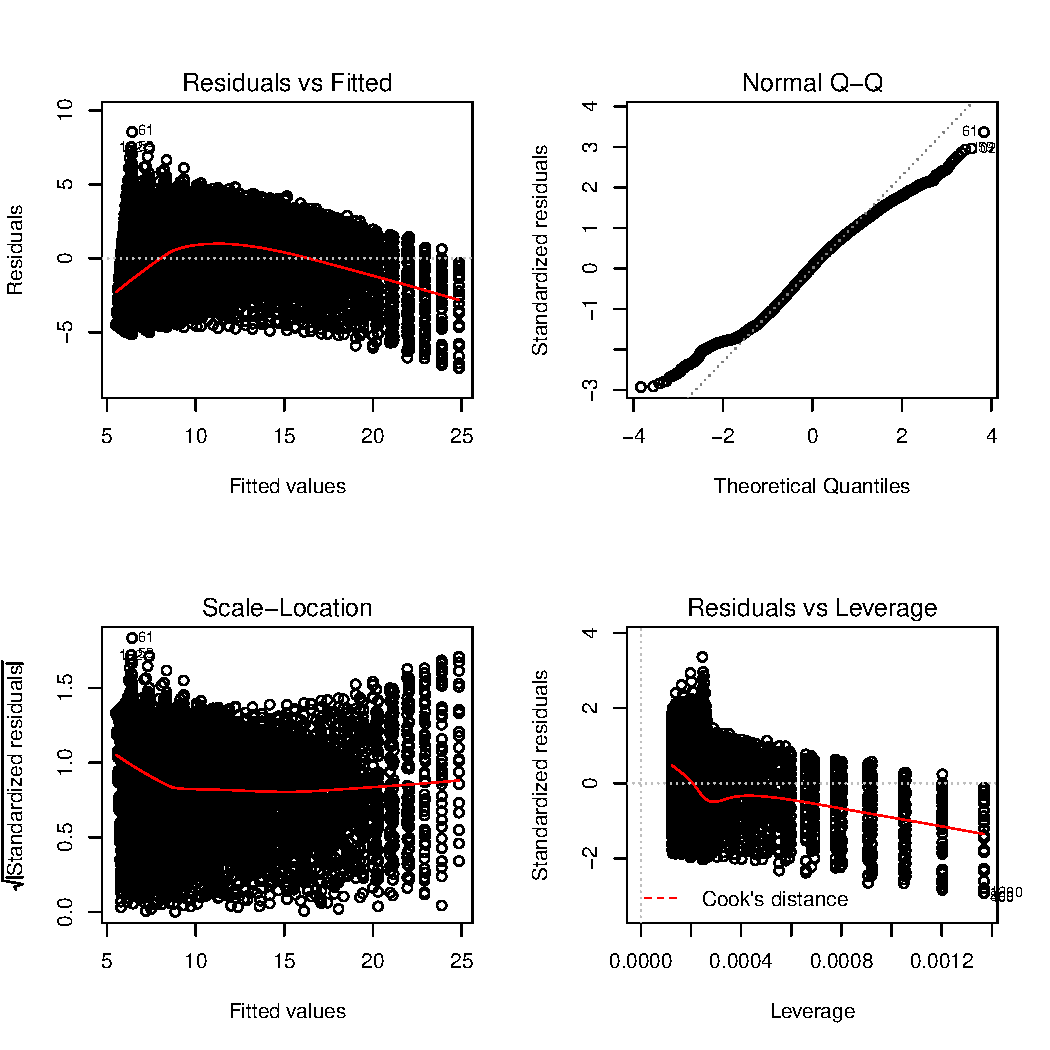
\includegraphics[width=\linewidth]{../../Results/Simulation/AreaSpeciesLmPlot_1.pdf}
    \caption{maxArea = 225 units}
  \end{subfigure}
  \begin{subfigure}[b]{0.4\linewidth}
    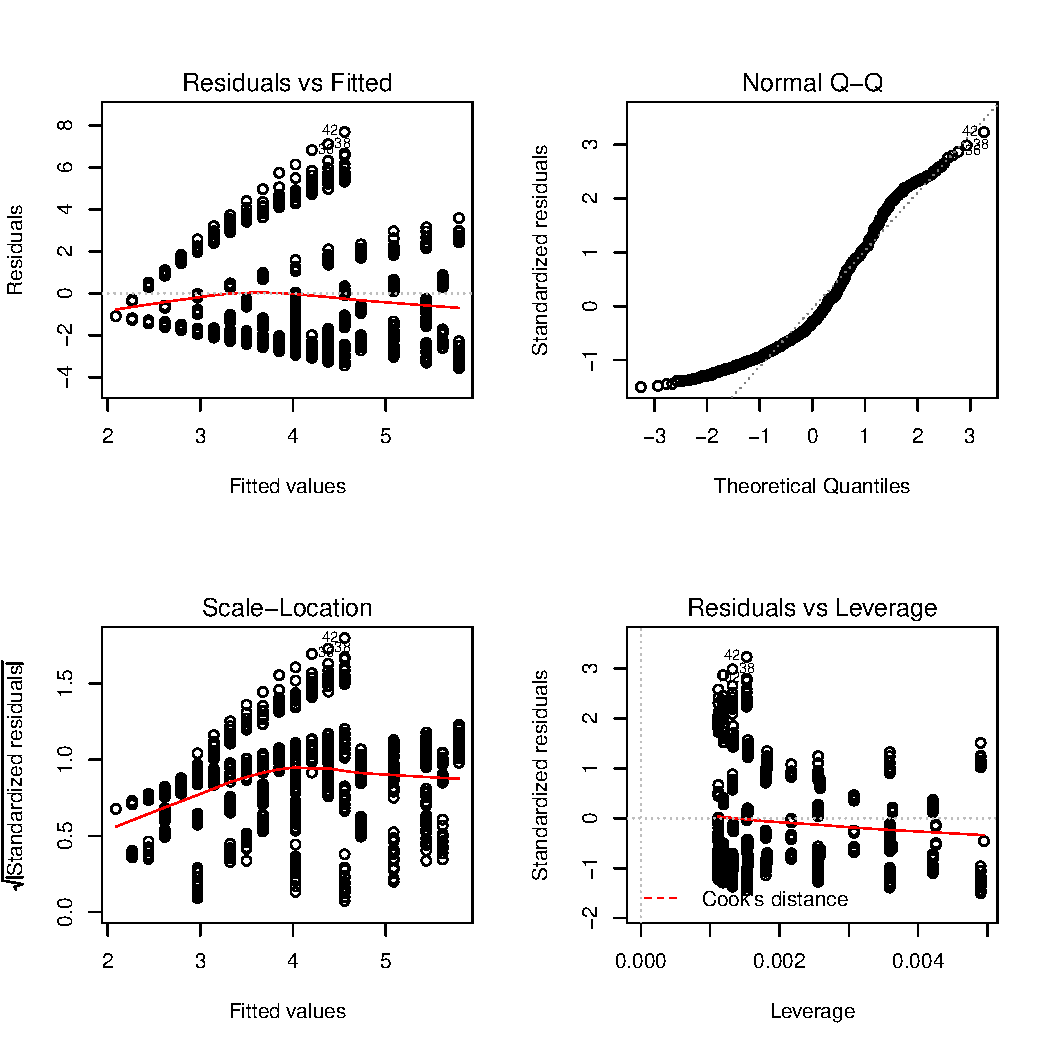
\includegraphics[width=\linewidth]{../../Results/Simulation/AreaSpeciesLmPlot_10.pdf}
    \caption{maxArea = 22 units}
  \end{subfigure}
  \caption{Model validation: Diagnostic plots of area and species richness linear models with full data set and reduced data set}
  \label{fig:Model validation area/species LM}
\end{figure}

Visual inspection of the residual vs fitted plot for the most reduced dataset showed fairly linear but non-constant variance (Figure 5 (b)). Higher fitted values had a greater residual range than lower fitted values. The normal Q-Q plot followed a relatively straight line. Diagnostics indicate the model continues to work fairly well for the data at lower island areas. \bigskip

The linear model result of species richness and z-transformed niches gave an r-squared value of 0.89 with a p-value $<$ 0.001 (Table 2). This indicated that niches had a positive, statistically significant relationship with species richness. \bigskip

\begin{figure}[h!]
  \centering
  \begin{subfigure}[b]{0.4\linewidth}
    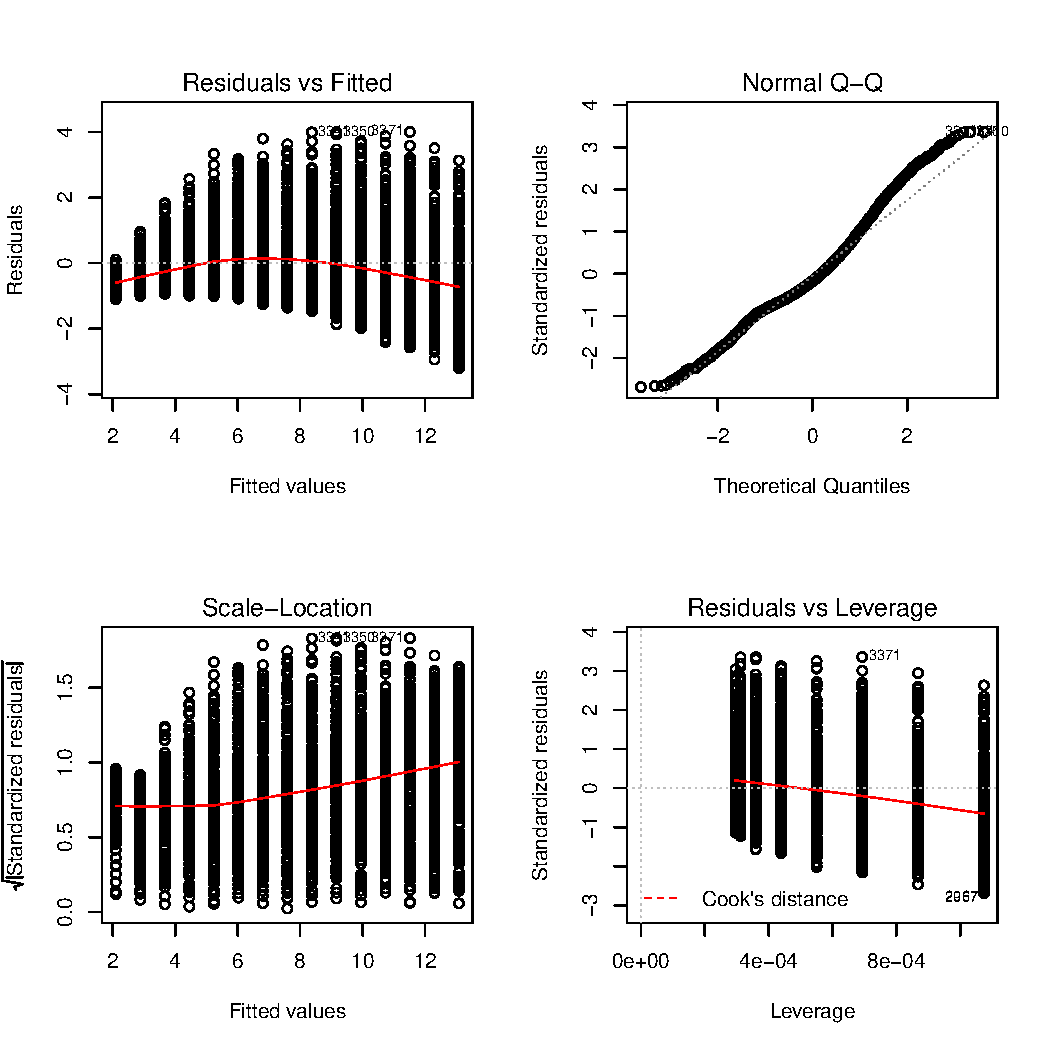
\includegraphics[width=\linewidth]{../../Results/Simulation/NicheSpeciesLmPlot_1.pdf}
    \caption{maxArea = 225 units}
  \end{subfigure}
  \begin{subfigure}[b]{0.4\linewidth}
    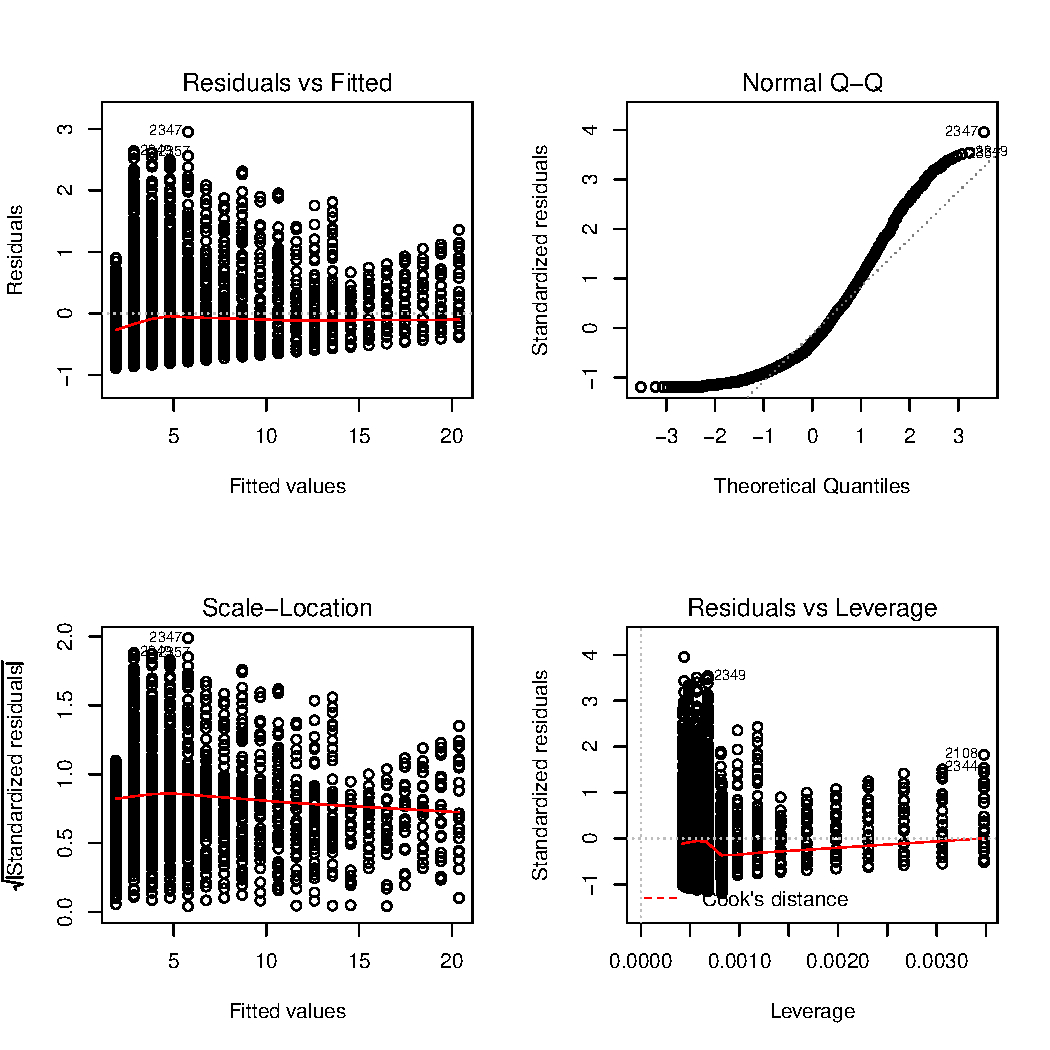
\includegraphics[width=\linewidth]{../../Results/Simulation/NicheSpeciesLmPlot_10.pdf}
    \caption{maxArea = 22 units}
  \end{subfigure}
  \caption{Model validation: Diagnostic plots of niche and species richness linear models with full data set and reduced data set}
  \label{fig:Model validation niche/species LM}
\end{figure}

Visual inspection of the residual vs fitted plot for the entire dataset showed fairly linear but non-constant variance (Figure 6 (a)). Higher fitted values had a greater residual range than lower fitted values. The normal Q-Q plot followed a relatively straight line. Diagnostics indicate the model works fairly well for the data. \bigskip

The r-squared value for niches/species richness linear model increased from 0.89 to 0.977 as maximum island area was reduced from 225 units to 22 units (Table 2). This indicated that number of niches had a stronger positive relationship with species richness as island area decreased. \bigskip

Visual inspection of the residual vs fitted plot for the most reduced dataset (Figure 6 (b)) showed fairly linear and randomly distributed variance. The normal Q-Q plot followed a relatively straight line.  Diagnostics indicate the model works fairly well for the data. \bigskip

\subsubsection{Multivariate Regression Analysis}

\begin{table}[h!]
\centering
\caption{Multiple regression analysis for z-transformed migration, area and niches}
\pgfplotstabletypeset[
    col sep=comma,
    ignore chars={",_}, %get rid of quote marks around my text and ignore underscores
    string type,
    every head row/.style={%
        before row={\hline
           % \multicolumn{2}{c}{incase you wanted a title above the column headers} & \\
        },
        after row=\hline
    },
    every last row/.style={after row=\hline},
    columns/maxArea/.style={column name=maxArea, column type=c},
    columns/Coefficients/.style={column name=Coefficients, column type=c},
    columns/Estimate/.style={column name=Estimate, column type=c},
    columns/standarderror/.style={column name=StandardError, column type=c},
    columns/tvalue/.style={column name=tValue, column type=c},
    columns/pvalue/.style={column name=pValue, column type=l}, %problem with less than sign
    columns/rsquared/.style={column name=rSquared, column type=c},
    columns/variate/.style={column name=Variate, column type=l},
    ]{../../Results/Simulation/MultiMaxMin.csv}
   \end{table}\bigskip
   
Multivariate analysis results for the whole dataset showed that the combined effects of number of niches, island area and migration rate gave an r-squared value of 0.972 (Table 3). The combined effects of niche and area gave an r-squared value of 0.961. This indicates that migration rate had a weak positive effect on species richness across the entire dataset.  \bigskip

\begin{figure}[h!]
  \centering
  \begin{subfigure}[b]{0.4\linewidth}
    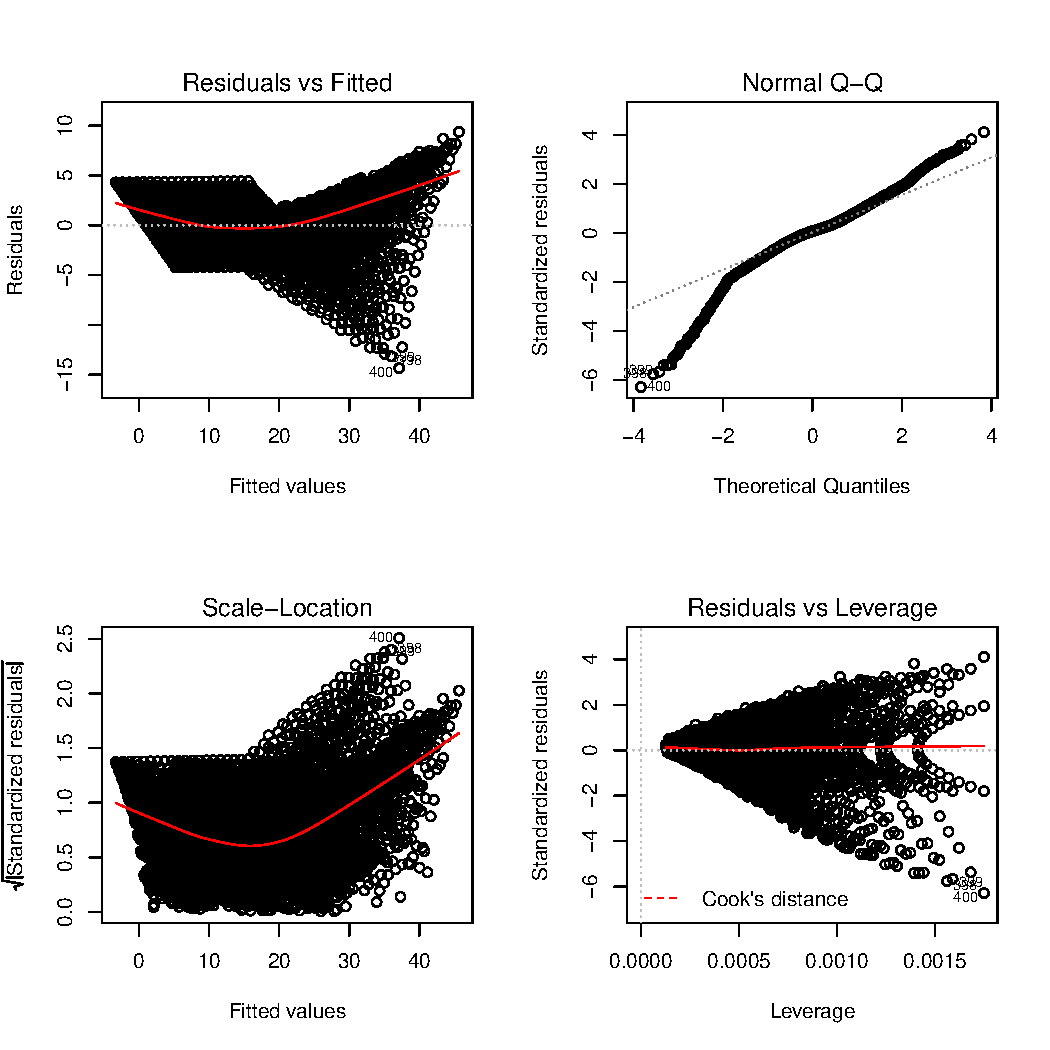
\includegraphics[width=\linewidth]{../../Results/Simulation/NicheAreaMigrationLmPlot_1.pdf}
    \caption{maxArea = 225 units}
  \end{subfigure}
  \begin{subfigure}[b]{0.4\linewidth}
    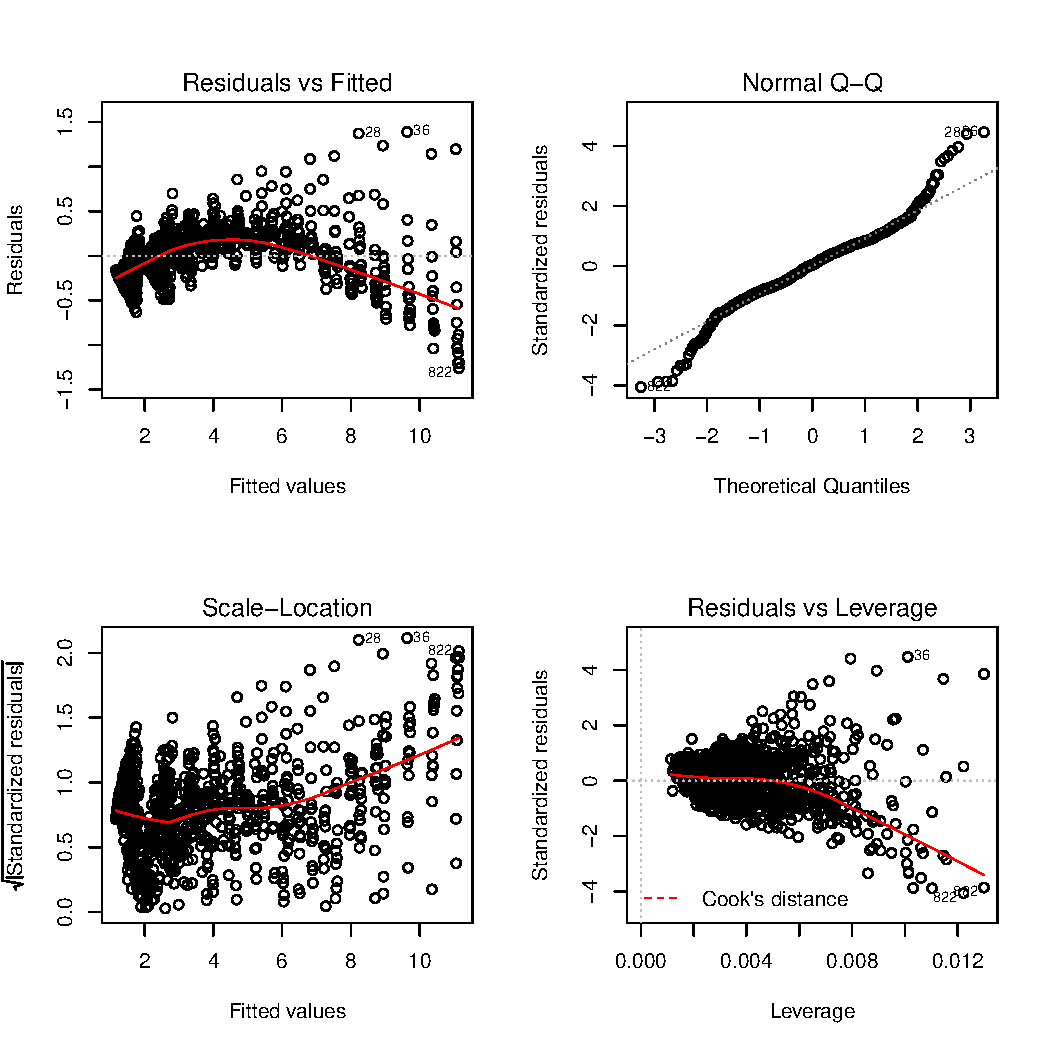
\includegraphics[width=\linewidth]{../../Results/Simulation/NicheAreaMigrationLmPlot_10.pdf}
    \caption{maxArea = 22 units}
  \end{subfigure}
  \caption{Model validation: Residuals plots of multivariate analysis of niche, area, migration and species richness with full data set (a) and reduced data set (b)}
  \label{fig:Model validation multivariate 1}
\end{figure}

\begin{figure}[h!]
  \centering
  \begin{subfigure}[b]{0.4\linewidth}
    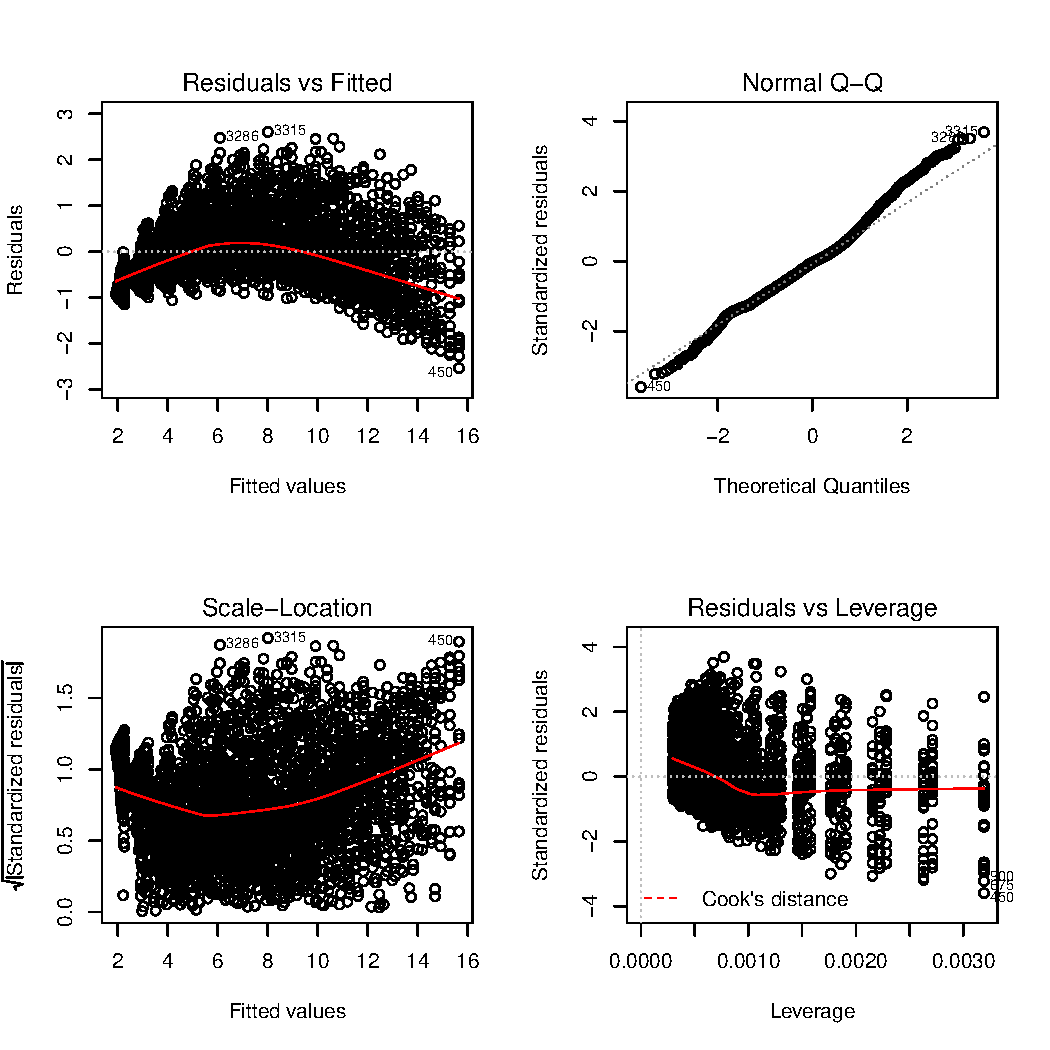
\includegraphics[width=\linewidth]{../../Results/Simulation/NicheAreaLmPlot_1.pdf}
    \caption{maxArea = 225 units}
  \end{subfigure}
  \begin{subfigure}[b]{0.4\linewidth}
    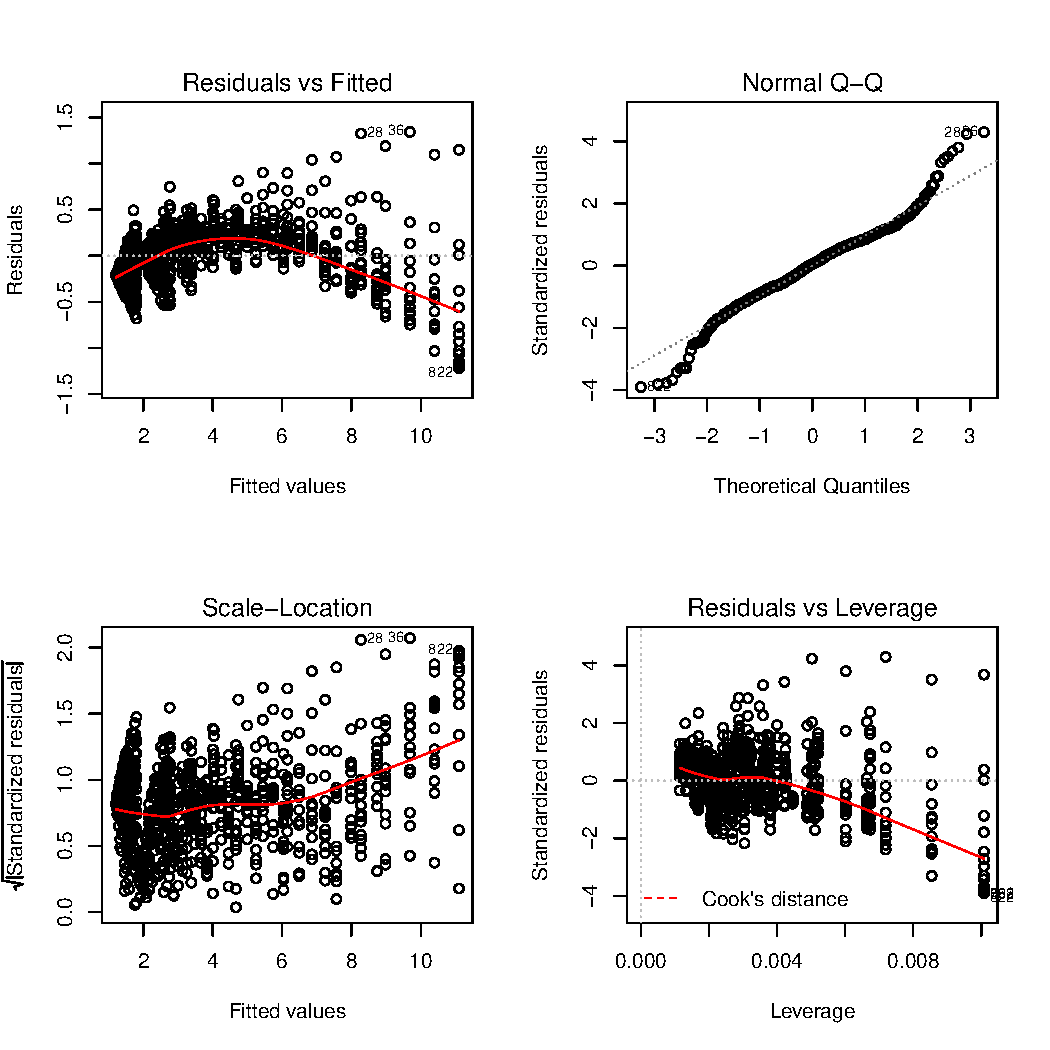
\includegraphics[width=\linewidth]{../../Results/Simulation/NicheAreaLmPlot_10.pdf}
    \caption{maxArea = 22 units}
  \end{subfigure}
  \caption{Model validation: Diagnostic plots of multivariate analysis of niche, area and species richness with full data set (a) and reduced data set (b)}
  \label{fig:Model validation multivariate 2}
\end{figure}


Visual inspection of the residual results for the multivariate analysis showed non-linear but fairly evenly distributed variance (Figure 7 (a)). The Q-Q plot follows a relatively straight line. \bigskip

Multivariate analysis results for the most reduced dataset showed that the combined effects of number of niches, island area and migration rate, gave an r-squared value of 0.985 (Table 3). The combined effects of niche and area gave an r-squared value of 0.985, indicating that migration rate had no effect on species richness at smaller island sizes. \bigskip

Visual inspection of the residual results for the reduce dataset show a non-linear and non-constant variance (Figure 7 (b)). The Q-Q plot deviates at the lowest and highest theoretical quantiles.   

\subsection{Simulation/Model Results}

\subsubsection{Outliers}

\begin{figure}[h!]
  \centering
  \begin{subfigure}[b]{0.4\linewidth}
    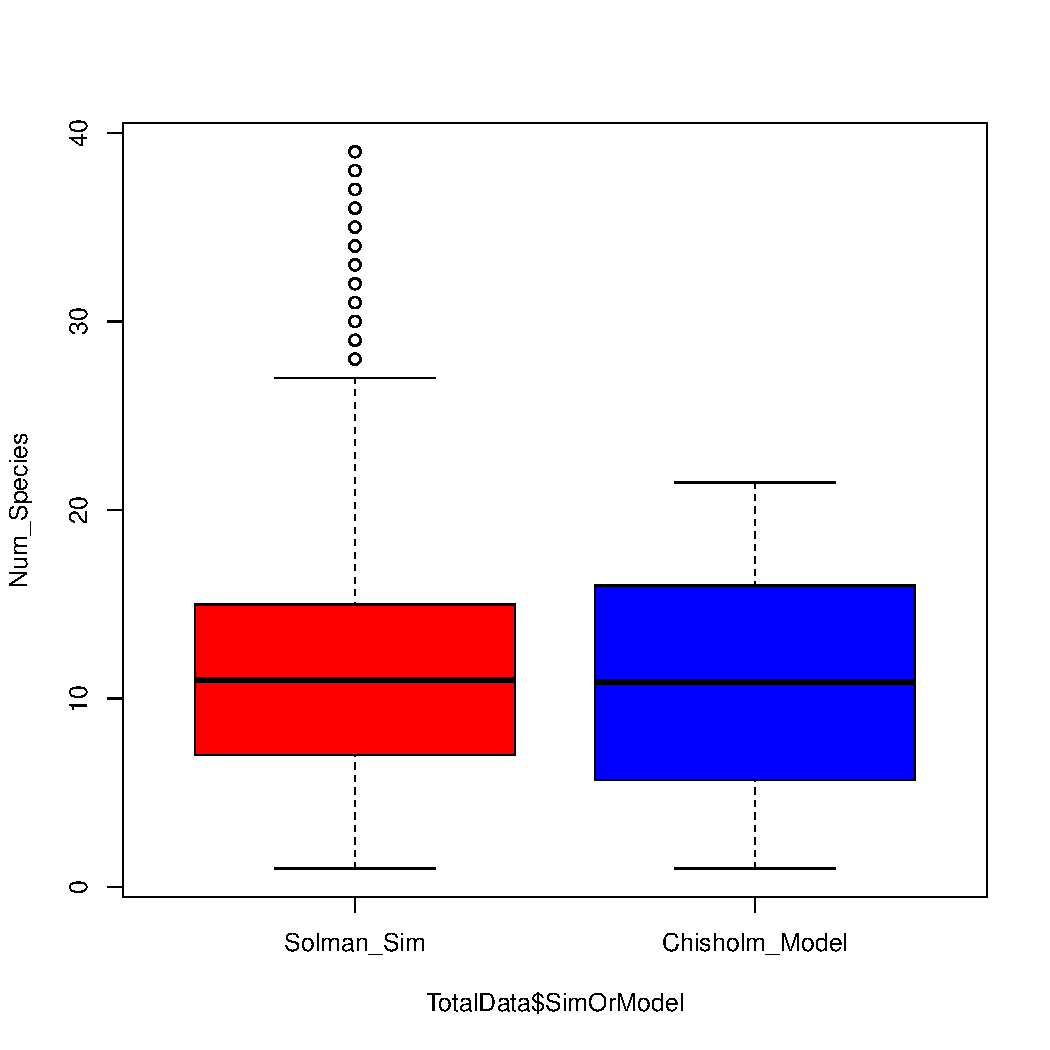
\includegraphics[width=\linewidth]{../../Results/Simulation/SolmanChisholmBoxplot_1.pdf}
    \caption{maxArea = 225 units}
  \end{subfigure}
  \begin{subfigure}[b]{0.4\linewidth}
    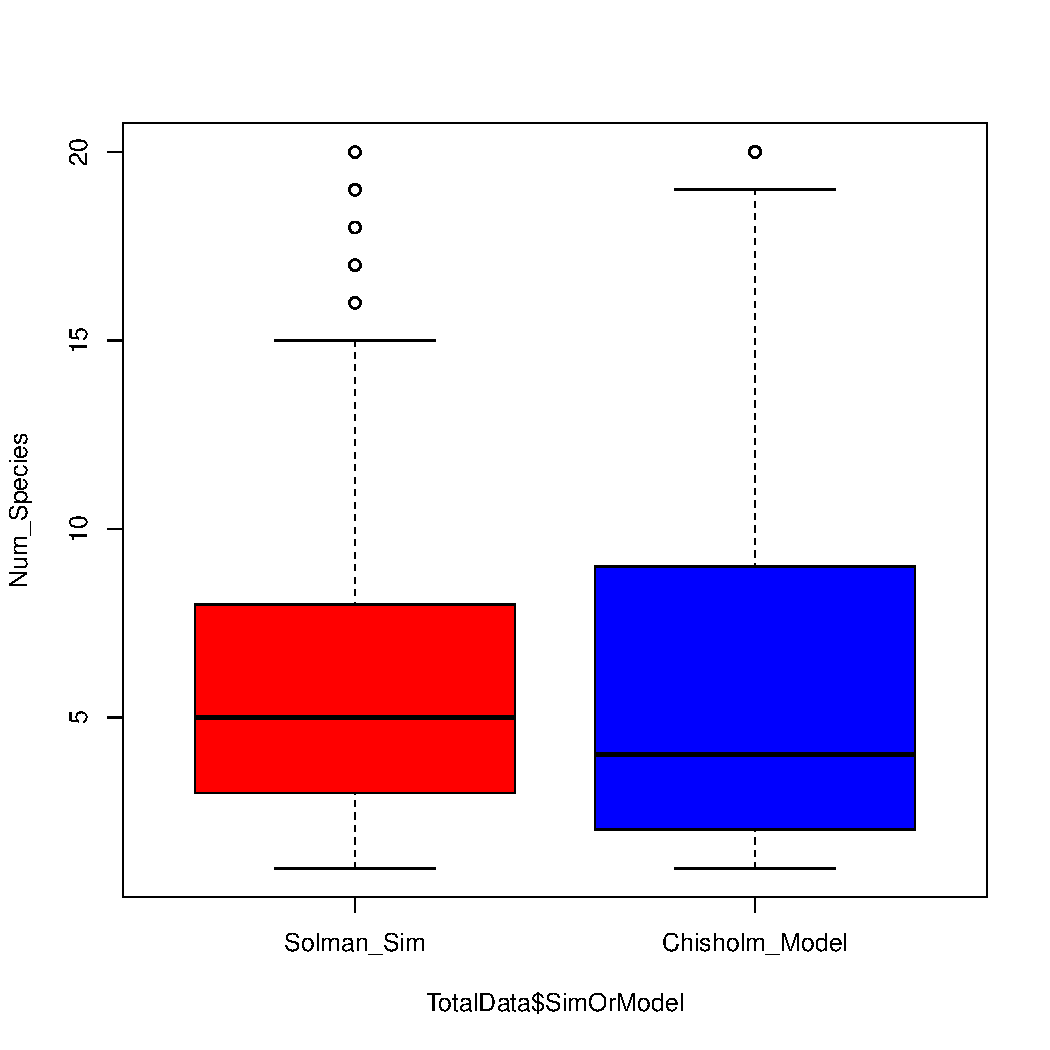
\includegraphics[width=\linewidth]{../../Results/Simulation/SolmanChisholmBoxplot_10.pdf}
    \caption{maxArea = 22 units}
  \end{subfigure}
  \caption{Boxplot of simulation and model estimation data for the full data set and area reduced data set}
  \label{fig:boxplots}
\end{figure}

When comparing boxplots of simulated and model estimated species richnesses, the simulation boxplot appeared to show outlying data points (Figure 9 (a)). On examining the data, the plotted points represented 569 islands that had species richness values greater than 20. As the number of islands present in this outlier group was so high, it was inappropriate to remove them from the data set as they represent a significant contrinution to the overall mean. Moreover, there was not a sudden jump in values from those within the quartile ranges of the boxplot to those indicated as outliers. It is for this reason the boxplot appears to be misleading.  \bigskip

Boxplots of the reduced data indicate outliers in both the simulation and model estimate datasets (Figure 9 (b)). 349 islands in the simulation data set had species richness $>$= 13 and 3000 islands in the model estimation dataset had species richness $>$=14. The outliers in this case do not appear to be random deviates from the data, but represent a considerable proportion of the overall dataset and are not removed from this analysis.  

\subsubsection{Mean, range, variance, standard deviation and standard error}

\begin{table}[h!]
\caption{Mean, range, variance, SD and SE for simulation and model estimates}
\centering
\pgfplotstabletypeset[
    col sep=comma,
    ignore chars={"}, %get rid of quote marks around my text
    string type,
    every head row/.style={%
        before row={\hline
           % \multicolumn{2}{c}{incase you wanted a title above the column headers} & \\
        },
        after row=\hline
    },
    every last row/.style={after row=\hline},
    columns/mean/.style={column name=Mean, column type=c},
    columns/range/.style={column name=Range, column type=c},
    columns/variance/.style={column name=Variance, column type=c},
    columns/standarddeviation/.style={column name=StandardDeviation, column type=c},
    columns/standarderror/.style={column name=StandardError, column type=c},
    columns/maxArea/.style={column name=maxArea, column type=c},
    columns/ModelOrSim/.style={column name=ModelOrSim, column type=l},
    ]{../../Results/Simulation/StatsEdit.csv}
   \end{table}\bigskip
    
For the full dataset, the mean number of species on simulated islands was 7.6 (SD 3.9, SE 0.007, range: 1-25) (Table 4).
The mean number of species estimated by the model directly was 8.1 (SD 4.4 , SE 0.007, range: 1-15.5). For the reduced island size dataset, the mean number of species on simulated islands was 4.0 (SD 2.7, SE 0.009, range: 1-15). The mean number of species estimated by the model directly was 4.5 (SD 3.7, SE 0.012, range: 1-15).

\subsubsection{Paired-sample t-Test}

\begin{table}[h!]
\caption{Paired-sample t-test for simulation data and model estimations}
\centering
\pgfplotstabletypeset[
    font={\small},
    begin table=\begin{longtable},
    end table=\end{longtable},
    col sep=comma,
    ignore chars={"}, %get rid of quote marks around my text
    string type,
    every head row/.style={%
        before row={\hline
           % \multicolumn{2}{c}{incase you wanted a title above the column headers} & \\
        },
        after row=\hline
    },
    every last row/.style={after row=\hline},
    columns/mean/.style={column name=MeanDifference, column type=c},
    columns/tvalue/.style={column name=tValue, column type=c},
    columns/pvalue/.style={column name=pValue, column type=l},
    columns/df/.style={column name=DF, column type=c},
    columns/conflow/.style={column name=ConfLow, column type=c},
    columns/confhigh/.style={column name=ConfHigh, column type=c},
    columns/method/.style={column name=Method, column type=l},
    columns/alternative/.style={column name=Alternative, column type=l},
    columns/maxArea/.style={column name=maxArea, column type=c},
    ]{../../Results/Simulation/pairedtMaxMin.csv}
   \end{table}\bigskip
   
The mean difference between simulation results and model estimations for the full dataset were -0.47, with a t-value of -125.64 and a p-value of $<$ 0.001 (DF 337499, CI low -0.48, CI high -0.47). The mean difference between simulation results and model estimations for the most reduced dataset were -0.51, with a t-value of -100.4 and a p-value of $<$ 0.001 (DF 89999, CI low -0.52, CI high 0.5).

\subsubsection{Non-Linear Least Squares Fitting}      
   
\begin{table}[h!]
\caption{NLLS fitting of Chisholm model to simulation data, parameter statistics}
\centering
\pgfplotstabletypeset[
    col sep=comma,
    ignore chars={"}, %get rid of quote marks around my text
    string type,
    every head row/.style={%
        before row={\hline
           % \multicolumn{2}{c}{incase you wanted a title above the column headers} & \\
        },
        after row=\hline
    },
    every last row/.style={after row=\hline},
    columns/terms/.style={column name=Terms, column type=c},
    columns/estimate/.style={column name=Estimate, column type=c},
    columns/standarderror/.style={column name=StandardError, column type=c},
    columns/statistic/.style={column name=Statistic, column type=c},
    columns/pvalue/.style={column name=pValue, column type=c},
    columns/rsquared/.style={column name=rSquared, column type=c},
    columns/migrationrate/.style={column name=MigrationRate, column type=c},
    columns/niches/.style={column name=Niches, column type=c},
     columns/numislands/.style={column name=NumIslands, column type=c},
    ]{../../Results/Simulation/NLLS/SumResults.csv}
   \end{table}\bigskip

\begin{figure}
 \centering
 \begin{subfigure}[b]{0.4\linewidth}
  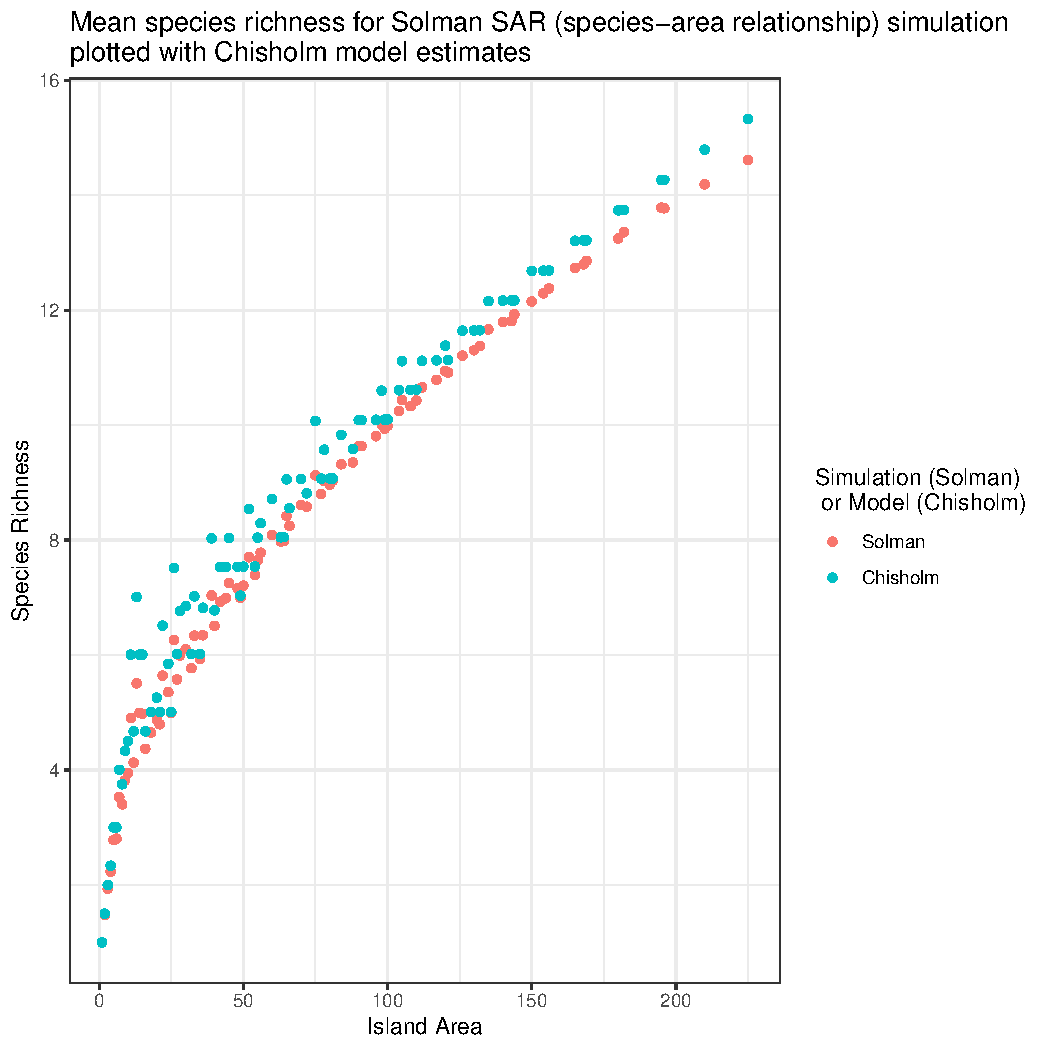
\includegraphics[width=\linewidth]{../../Results/Simulation/MeanResultsPlot.pdf}
   \caption{Direct estimations of species richness}
  \end{subfigure}
  \begin{subfigure}[b]{0.4\linewidth}
   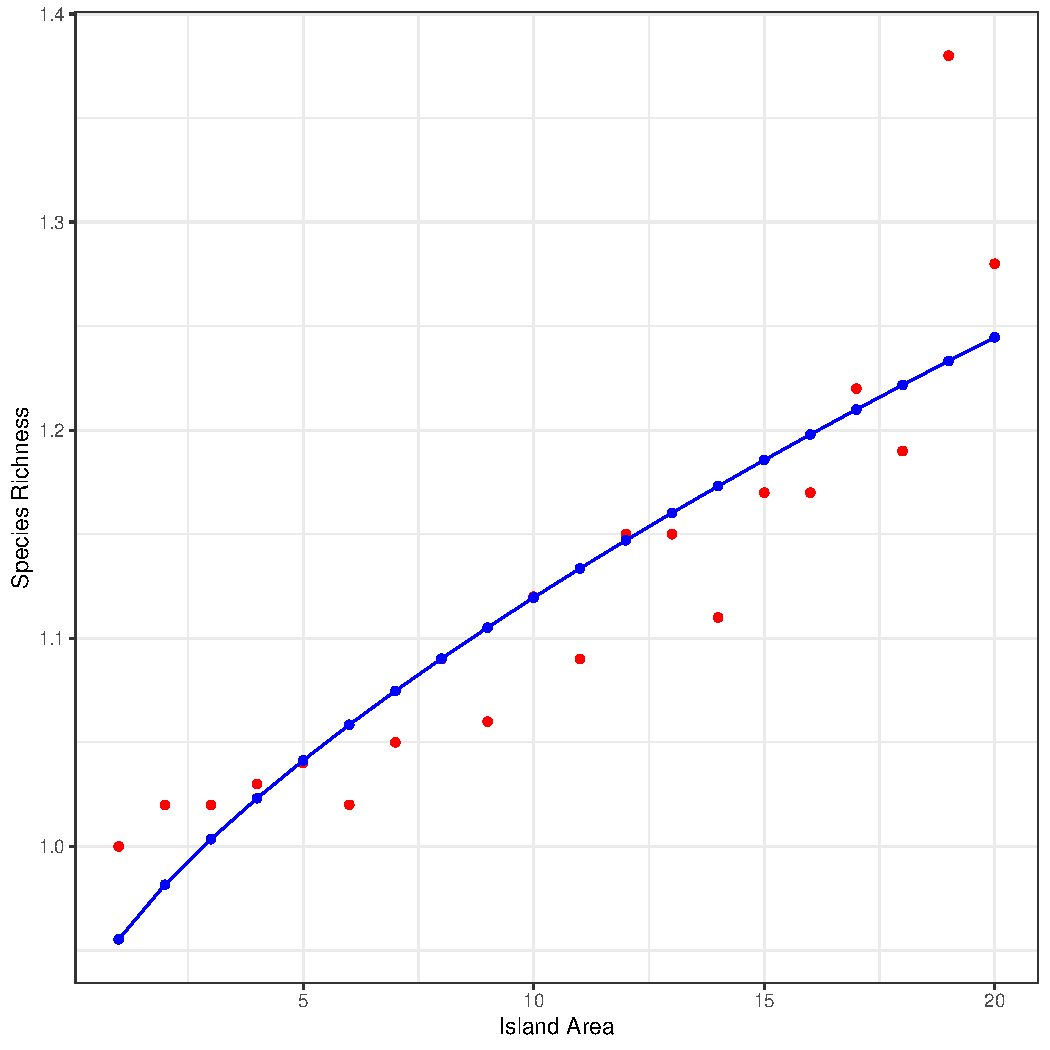
\includegraphics[width=\linewidth]{../../Results/Simulation/NLLS/Plot_1.pdf}
    \caption{NLLS estimations of species richness}
  \end{subfigure}
  \caption{Chisholm model estimations of species richness directly and through NLLS fitting}
  \label{fig:modelfitting}
\end{figure}

The total mean species richness estimated by the model using NLLS fitting was 8.15 (SD 3.26, SE 0.35, range: 1.81 - 14.44). The total mean species richness for the simulation was 8.15 (SD 3.28, SE 0.35, range: 1 - 14.61) (Table 6). The R-squared value of the fitting was 0.99, which suggests 99\% of the variation in species richness in the simulation was explained by the model. 
The estimates theta for the simulation data was 21.7. The estimated m0 for the mean simulation data was 0.3, whilst the mean m0 was 1.3. The model estimated mean number of niches for the simulation data was 2.3, whilst the mean number of niches for the data was 8.5 (Table 7).
  Visual inspection of the direct model estimations and NLLS fitting reveal both were successful in predicting species richness on the simulated islands (Figure 10). However, the NLLS model fitting more closely follows the species richness data produced by the simulation.
  


\end{document}